\subsubsection{Postprocessing spherical 3D convection}
\label{sec:cookbooks-shell_3d_postprocess.prm}
\textit{This section was contributed by Jacqueline Austermann, Ian Rose, and Shangxin Liu}


There are several postprocessors that can be used to turn the velocity
and pressure solution into quantities that can be compared to surface
observations. In this cookbook (\url{cookbooks/shell_3d_postprocess/shell_3d_postprocess.prm})
we introduce two postprocessors: dynamic topography and the geoid.
We initialize the model with a harmonic
perturbation of degree 4 and order 2 and calculate the
instantaneous solution. Analogous to the previous setup we use a spherical
shell geometry model and a simple material model.

The relevant section in the input file that determines the postprocessed
output is as follows:

\lstinputlisting[language=prmfile]{shell_3d_postprocess.part.prm.out}

This initial condition results in distinct flow cells that cause local up- and
downwellings (Figure~\ref{fig:pp}). This flow deflects the top and bottom boundaries
of the mantle away from their reference height, a process known as dynamic topography.
The deflection of the surfaces and density perturbations within the mantle also
cause a perturbation in the gravitational field of the planet relative to the
hydrostatic equilibrium ellipsoid.

\paragraph{Dynamic topography at the surface and core mantle boundary.}
Dynamic topography is calculated at the surface and bottom of the domain
through a stress balancing approach where we assume that the radial stress at
the surface is balanced by excess (or deficit) topography. We use the
consistent boundary flux (CBF) method to calculate the radial stress
at the surface \cite{ZGH93}. For the
bottom surface we define positive values as up (out)
and negative values are down (in), analogous to the deformation of the upper
surface. Dynamic topography can be outputted in text format (which writes the
Euclidean coordinates followed by the corresponding topography value) or as
part of the visualization. The upwelling and downwelling flow along the
equator causes alternating topography high and lows at the top and
bottom surface (Figure~\ref{fig:pp}).
In Figure~\ref{fig:pp} c, d we have subtracted the mean dynamic topography from
the output field as a postprocessing step outside of \aspect{}. Since mass is
conserved within the Earth, the mean dynamic topography
should always be zero, however, the outputted values might not fulfill this
constraint if the resolution of the model is not high enough to provide an
accurate solution. This cookbook only uses a refinement of 2, which is relatively
low resolution.

\paragraph{Geoid anomalies.}
Geoid anomalies are perturbations of the gravitational equipotential surface that
are due to density variations within the mantle as well as deflections of the
surface and core mantle boundary. The geoid anomalies are calculated using a spherical
harmonic expansion of the respective fields. The user has the option to specify the
minimum and maximum degree of this expansion. By default, the minimum degree is
2, which conserves the mass of the Earth (by removing degree 0) and chooses the
Earth's center of mass as reference frame (by removing degree 1).
In this model, downwellings coincide with lows in the geoid anomaly. That
means the mass deficit caused by the depression at the surface is not
fully compensated by the high density material below the depression that
drags the surface down. The geoid postprocessor uses a spherical harmonic
expansion and can therefore only be used with the 3D spherical shell geometry model.


\begin{figure}
  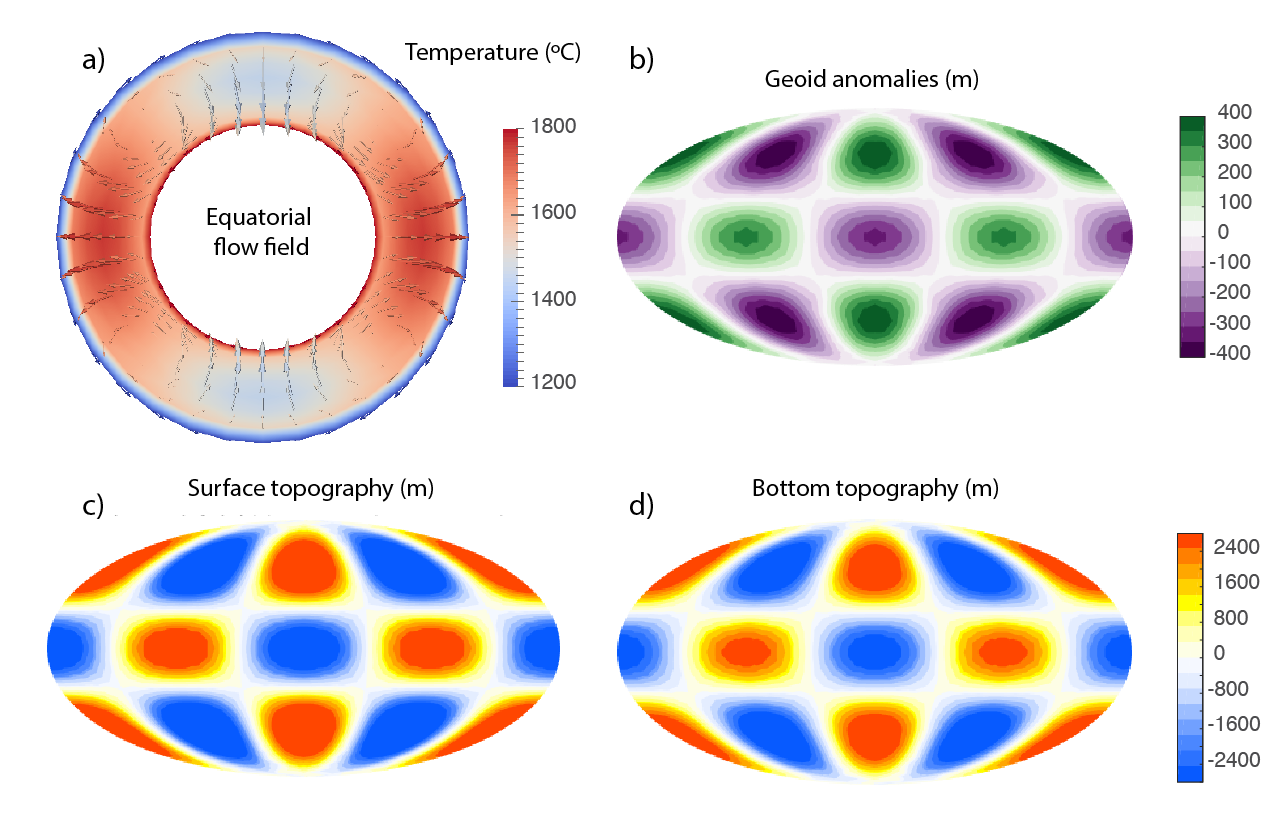
\includegraphics[width=\textwidth]{postprocess_cookbook-01.png}
  \hfill
  \caption{\it Panel (a) shows an equatorial cross section of the temperature distribution and
  resulting flow from a harmonic perturbation. Panel (b) shows the resulting geoid, and panels
  (c) and (d) show the resulting surface and bottom topography. Note that we have subtracted
  the mean surface and bottom topography in the respective panels (c and d) as a postprocessing
  step outside of Aspect.
  }
  \label{fig:pp}
\end{figure}

